%
% Thesis - Chapter 1
% Lakshitha de Silva
% School of Computer Science
% University of St Andrews, Scotland, UK
% 2014
%


\chapter{Introduction}
<Chapter Abstract>

\section{Overview}


\section{Central claims}


\section{Motivation}


\section{Main contributions}


\section{Organisation of Dissertation}
A short description of each chapter in this thesis is given below.

\begin{description}
\item[Chapter 1] gives an introduction to this dissertation .. bla bla bla

\item[Chapter 2] presents the background survey .. bla bla bla
\end{description}


\section{Examples}

\subsection{Citing References}
References are used in the following paragraph.

Architecture erosion and its effects are widely discussed in literature. Perry and Wolf \cite{Perry1992} differentiate \emph{architecture erosion} from \emph{architecture drift} as follows: erosion results from violating architectural principles while drift is caused by insensitivity to the architecture. As the underlying causes for both are the same, we will not consider this difference for the purpose of our survey. Additionally, the notion of software architecture erosion is discussed using a number of different terms such as architectural degeneration \cite{Hoch2003}, software erosion \cite{Dalgar2009}, design erosion \cite{Gurp2002}, architectural decay \cite{Riaz2009}, design decay \cite{Izur2007}, code decay \cite{Eick2001,String2006} and software entropy \cite{Jacob1992}. 


\subsection{Tables}
Tables have been configured to use the \emph{booktabs} package which gives professionally typeset tables. Two examples are shown below.

\begin{table*}[h]\small
	\centering
	\begin{tabulary}{\textwidth}{lp{3pt}J}
		\toprule
		Strategy && Contribution towards controlling erosion \\
		\midrule
		Architecture Design Documentation & \RIGHTarrow & Records architecture design and rationale with the intent of disseminating architectural knowledge to a wider audience and provides a point of reference for developers throughout system evolution. \\ [7pt]
		Architecture Analysis & \RIGHTarrow & Uncovers weaknesses in the intended architecture, in particular, sensitive points which can be easily violated in the implementation.  \\ [7pt]
		Architecture Conformance Monitoring & \RIGHTarrow & Establishes the means to verify whether the implementation is faithful to the intended architecture during both the development and subsequent maintenance phases of a system. \\ [7pt]
		\bottomrule
	\end{tabulary}
	\caption{Controlling architecture erosion with process-oriented strategies}
	\label{tab:process-oriented}
\end{table*}

\begin{table}[h]
	\centering
	\begin{tabular}{llll} 
		\toprule
		Run 		& Framework unplugged ($\mu$s)	& Using probes	($\mu$s) & Using JDI ($\mu$s)	\\
		\midrule
		1		& 108,644			& 143,002				& 488,018		\\
		2		& 107,929			& 141,185				& 486,951		\\
		3		& 107,319			& 141,274				& 482,206		\\
		4		& 106,054			& 142,333				& 479,477		\\
		\midrule
		Average	& 107,487			& 141,949 (+30.9\%)		& 484,163 (+345.6\%)	\\
		\bottomrule
	\end{tabular}
	\caption{A comparison of performance impact between the use of JDI and instrumentation probes.}
	\label{tab:performance}
\end{table}


\newpage
\subsection{Lists}
An example of an itemised list.

\begin{itemize}
\item \textbf{Naming conventions from architectural to programming constructs.} For example, a component in the architecture is implemented by a class of the same name. Blah blah blah.

\item \textbf{Combining architecture and implementation in a single artefact.} Conformance checks are minimised or not required in such systems since architecture and implementation are combined in one specification.
\end{itemize}

An example of an enumerated list.

\begin{enumerate}
\item \textbf{Initialise the static analyser.} Provide the compiled Java code of the target application to Structure101 to begin its static analysis process.

\item \textbf{Analyse the Java bytecode.} Setup Structure101 to perform detailed analysis of the Java bytecode that also includes exploring method invocations among Java types.
\end{enumerate}


\subsection{Figures}
An example showing how to include figures. Figure \ref{fig:eventdriven} is taken from a pdf file which gives very good quality and therefore should be used for diagrams as much as possible.

\begin{figure}[h]
	\centering
	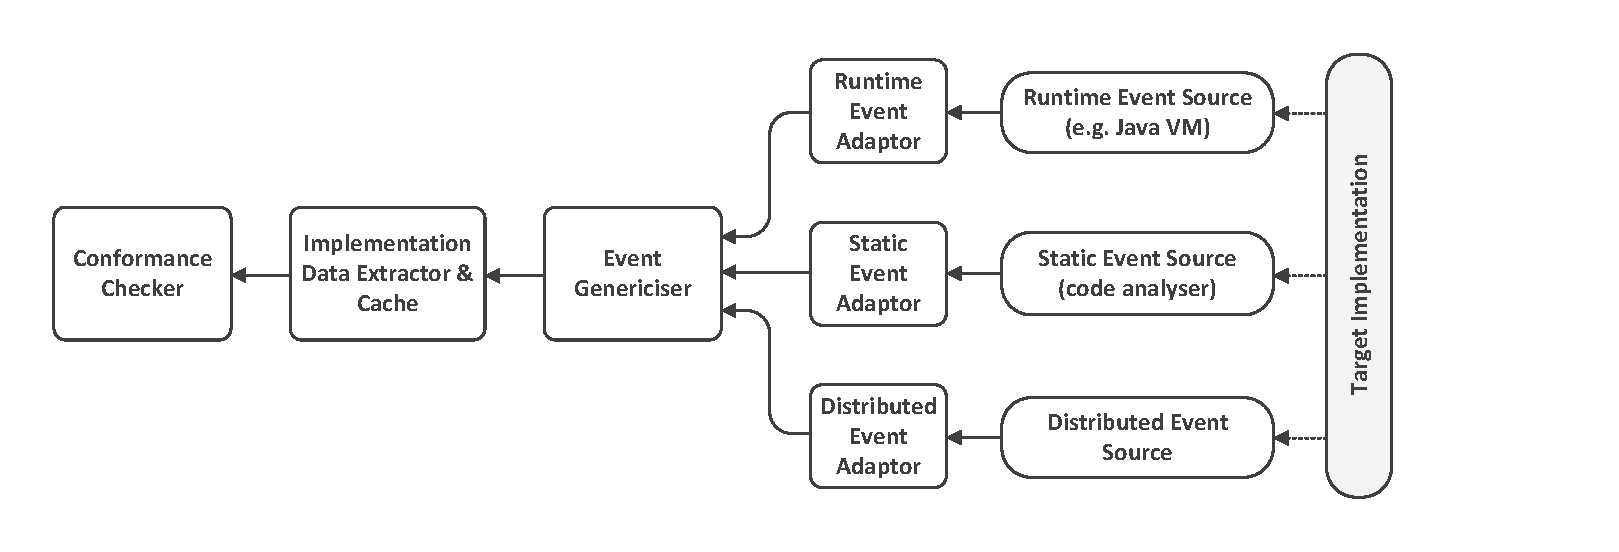
\includegraphics[width=\textwidth,trim=20 16 96 16]{fig-eventdriven.pdf}
	\caption{The event-driven process used for tapping implementation data}
	\label{fig:eventdriven}
\end{figure}


\newpage
\subsection{Code Listings}
An example of an inline code listing.
\begin{lstlisting}[caption={Hello World in Java},label=lst:javahello]
class HelloWorldApp {
	public static void main(String[] args) {
		System.out.println("Hello World!");		// Display messages
	}
}
\end{lstlisting}

Program code typeset from as an external file is shown in Listing \ref{lst:classtrans}. This also shows how to include line numbers.
\lstinputlisting[caption={Java class transformer},label=lst:classtrans,numbers=left]{
	chap1/src-example.java
}


\newpage
\subsection{Console Output}

\begin{lstlisting}[style=console]
John:/ $ ls -l
total 16437
drwxrwxr-x+ 52 root  admin     1768 10 Jan 13:21 Applications
drwxr-xr-x   3 root  wheel      102 27 Dec 18:01 Developer
drwxr-xr-x+ 66 root  wheel     2244  9 Jan 18:28 Library
drwxr-xr-x@  2 root  wheel       68 25 Aug 01:15 Network
drwxr-xr-x+  4 root  wheel      136 18 Dec 13:58 System
drwxr-xr-x   6 root  admin      204 18 Dec 14:16 Users
drwxrwxrwt@  4 root  admin      136 13 Jan 17:50 Volumes
drwxr-xr-x@ 39 root  wheel     1326 18 Dec 14:00 bin
drwxrwxr-t@  2 root  admin       68 25 Aug 01:15 cores
dr-xr-xr-x   3 root  wheel     4228 11 Jan 11:31 dev
lrwxr-xr-x@  1 root  wheel       11 18 Dec 13:46 etc -> private/etc
dr-xr-xr-x   2 root  wheel        1 13 Jan 16:10 home
-rwxr-xr-x@  1 root  wheel  8393256 20 Sep 06:22 mach_kernel
dr-xr-xr-x   2 root  wheel        1 13 Jan 16:10 net
drwxr-xr-x@  6 root  wheel      204 18 Dec 14:06 private
drwxr-xr-x@ 62 root  wheel     2108 18 Dec 14:02 sbin
lrwxr-xr-x@  1 root  wheel       11 18 Dec 13:47 tmp -> private/tmp
drwxr-xr-x@ 13 root  wheel      442 19 Dec 11:59 usr
lrwxr-xr-x@  1 root  wheel       11 18 Dec 13:47 var -> private/var
\end{lstlisting}


\subsection{Defining accronyms}
Blah blah blah \gls{vm} blah  blah blah blah and \gls{jvm}. However, blah blah blah, \gls{jvm} and also any other \gls{vm} blah blah blah. The \gls{jre} blah blah blah blah \gls{jvm} and blah blah blah blah \gls{cpu} blah blah blah blah blah. Typically, most blah blah blah \gls{ide} blah blah blah blah, however most \glspl{ide} blah blah blah blah blah blah blah.




